\section{Organisation usuelle d'un projet d'annotation}
\label{section:2.2-ORGANISATION-ANNOTATION}
	
	%%% Introduction: 
	Dans la section précédente, nous avons présenté l'importance d'avoir des données annotées pour entraîner d'un modèle de \textit{Machine Learning}.
	Maintenant, nous allons détailler la préparation et l'organisation de cette tâche d'annotation, et identifier les compétences nécessaires aux intervenants du projet.
	
	
	%%%
	%%% Subsection 2.2.1: Étapes clés du cycle d'annotation.
	%%%
	\subsection{Étapes clés du cycle d'annotation}
	\label{section:2.2.1-ORGANISATION-ANNOTATION-ETAPES-CLES}
		% \cite{pustejovsky-stubbs:2012:natural-language-annotation} et \cite{stubbs:2013:methodology-using-professional} formalisation MATTER
		% \cite{finlayson-erjavec:2016:overview-annotation-creation}
		% \cite{bonneau-maynard-etal:2005:semantic-annotation-french} première tentative de réviser un modèle, \cite{voormann-gut:2008:agile-corpus-creationa} formalisation du besoin de réviser sa modélisation
		
		%%% Introduction au cycle MATTER.
		Une référence en matière d'organisation de projet d'annotation est proposé par \cite{pustejovsky-stubbs:2012:natural-language-annotation} : les auteurs y formalisent la conception et l'amélioration \textbf{cyclique} d'un modèle de \textit{Machine Learning}.
		Ce cycle est appelé cycle \texttt{MATTER} en référence aux six étapes de conception qui le composent : \textit{\textbf{M}odelize}, \textit{\textbf{A}nnotate}, \textit{\textbf{T}rain}, \textit{\textbf{T}est}, \textit{\textbf{E}valuate} et \textit{\textbf{R}evise}.
		Ces étapes sont schématisées en \textsc{Figure~\ref{figure:2.2.1-ORGANISATION-ANNOTATION-ETAPES-CLES-MATTER}} et nous détaillons chacune d'entre elles ci-dessous.
		%
		\begin{figure}[!htb]
			\centering
			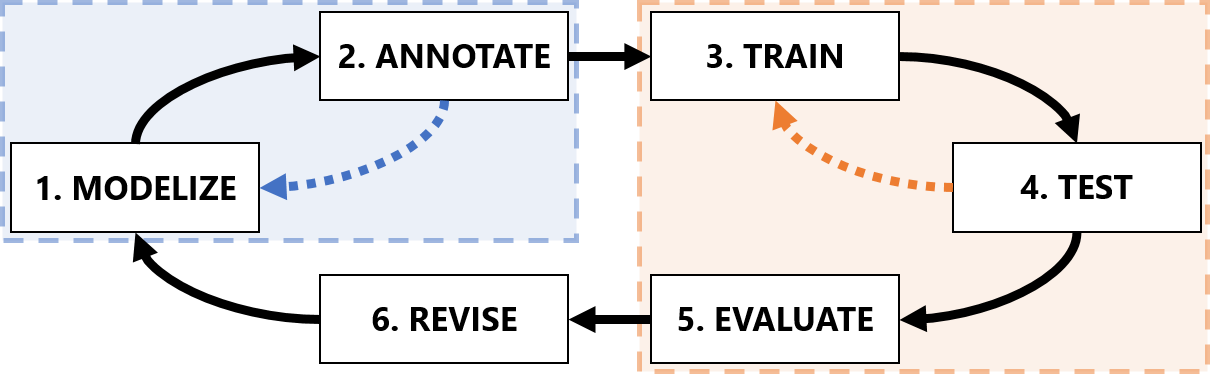
\includegraphics[width=0.95\textwidth]{figures/etatdelart-pustejovsky-2012-cycle-matter-mama-tt}
			\caption{
				Cycle \texttt{MATTER} structurant un projet d'annotation en six étapes principales: \textit{\textbf{M}odelize}, \textit{\textbf{A}nnotate}, \textit{\textbf{T}rain}, \textit{\textbf{T}est}, \textit{\textbf{E}valuate} et \textit{\textbf{R}evise}.
			}
			\label{figure:2.2.1-ORGANISATION-ANNOTATION-ETAPES-CLES-MATTER}
		\end{figure}
		
		% Collecte
		% M, A, mais aussi MAMA
		% TT, mais aussi Train Dev Test, puis Evaluate
		% Revise
		
		%%% 2.2.1.A. Concevoir la base d'apprentissage (\textbf{M}odelize}, \textit{\textbf{A}nnotate}).
		\paragraph{Concevoir la base d'apprentissage (\textit{\textbf{M}odelize}, \textit{\textbf{A}nnotate}).}
		
			% a. Collecte de données.
			Pour concevoir une base d'apprentissage, il faut d'abord disposer de données représentant le problème à modéliser.
			Une phase de collecte est alors organisée : cette collecte peut se baser sur des avis éclairés d'experts du problème, sur des extractions de bases de données ou de sites internet à disposition, sur des enquêtes réalisées après d'utilisateurs finaux, ...
			Comme nous l'avons vu précédemment, ces données brutes ont ensuite besoin d'être annotées pour pouvoir être exploitées.
			
			% b. Modelisation des données.
			\todo[inline]{
				pas de précipitation ; \\
				faire des règles d'annotations (\textit{\textbf{M}odelize}) ; \\
				pour produire un travail de qualité. \\
				Ces règles peuvent concerner :
				%\begin{itemize}
				%	\item objectif de l'annotation;
				%	\item pertinence de la données par rapport à l'objectif pour trier la collecte;
				%	\item format et valeurs possibles de l'annotation;
				%	\item documentation et définition des annotations
				%\end{itemize} 
				Il est important de faire attention à :
				%\begin{itemize}
				%	\item generalité vs spécificité;
				%	\item réutilisabilité;
				%	\item faisabilité ?
				%\end{itemize}
				exemple.
			}
			
			% c. Annotation
			\todo[inline]{
				réalisation en tant que telle
			}
			
			% d. Mini-cycle MAMA.
			\todo[inline]{
				remise en cause du modèle, affinage, ...
			}
			
			% e. Exemple
			\todo[inline]{
				Exemple à présenter
			}
		
		%%% 2.2.1.B. Concevoir le modèle (\textit{\textbf{T}rain}, \textit{\textbf{T}est}, \textit{\textbf{E}valuate}).
		\paragraph{Concevoir le modèle (\textit{\textbf{T}rain}, \textit{\textbf{T}est}, \textit{\textbf{E}valuate}).}
			\todo[inline]{a rédiger}
		
		%%% 2.2.1.C. Revoir la base d'apprentissage (\textit{\textbf{R}evise}).
		\paragraph{Revoir la base d'apprentissage (\textit{\textbf{R}evise}).}
			\todo[inline]{a rédiger}
	
	
	%%%
	%%% Subsection 2.2.2: Portraits des acteurs intervenant sur un projet d'annotation.
	%%%
	\subsection{Portraits des acteurs intervenant sur un projet d'annotation}
	\label{section:2.2.2-ORGANISATION-ANNOTATION-ACTEURS}
		\todo[inline]{SECTION: À RÉDIGER: \\
			- Acteurs: Objectifs, Rôles, Compétences, ... ; \\
			~~~~ - Axe métier (business expert) ; \\
			~~~~ - Axe technique (data scientist) ; \\
			~~~~ - Axe manipulation (data analyst) ; \\
			~~~~ - Axe projet (project leader) ;
		}
	
	
	%%%
	%%% Subsection 2.2.3: Exemples de logiciels utilisés pour annoter.
	%%%
	\subsection{Exemples de logiciels utilisés pour annoter}
	\label{section:2.2.3-ORGANISATION-ANNOTATION-LOGICIELS}
		\todo[inline]{SECTION: À RÉDIGER: \\
			- Outils: Liste, Avantages, Inconvénients, Fonctionnalités ;
			~~~~ - Excel
			~~~~ - prodigy
				% - Glozz [Widlöcher & Mathet, 2009] http://www.glozz.org/
				% - Callisto [Day et al., 2004]
				% - MMAX2 [Müller, 2006] https://github.com/ottiram/MMAX2
				% - PALinkA [Orăsan, 2003]
				% - Gate [Cunningham_2022] https://gate.ac.uk/
				% - Brat [Stenetorp et al., 2012] http://brat.nlplab.org/
				% - WebAnno [Yimam et al., 2013] https://webanno.github.io/webanno/
				% - Inception [Klie et al., 2018] https://inception-project.github.io/
		}
	
	
	% Conclusion.
	\begin{leftBarSummary}
		\begin{todolist}
			\item[\itemok] Un projet d'annotation s'organise généralement en cycle (\texttt{MATTER}) au cours duquel l'annotateur créé une représentation mentale des données, réalise son annotation, entraîne son modèle, puis révise sa représentation mentale des données en fonction des performances du modèle obtenu.
			\item[\itemok] Un tel projet d'annotation nécessite une diversité de connaissances et de compétences (\textit{connaissances métiers, connaissances techniques, maîtrise de l'apprentissage automatique, ...}), faisant ainsi collaborer un grand nombre d'acteurs qualifiés pour une ou plusieurs phase du cycle d'annotation.
		\end{todolist}
	\end{leftBarSummary}